\paragraph{Sơ đồ tuần tự luồng đăng ký tài khoản bằng email}

Luồng nghiệp vụ này mô tả
chi tiết quá trình đăng ký tài khoản mới
sử dụng địa chỉ Email và mật khẩu.

\begin{figure}[H]
\centering
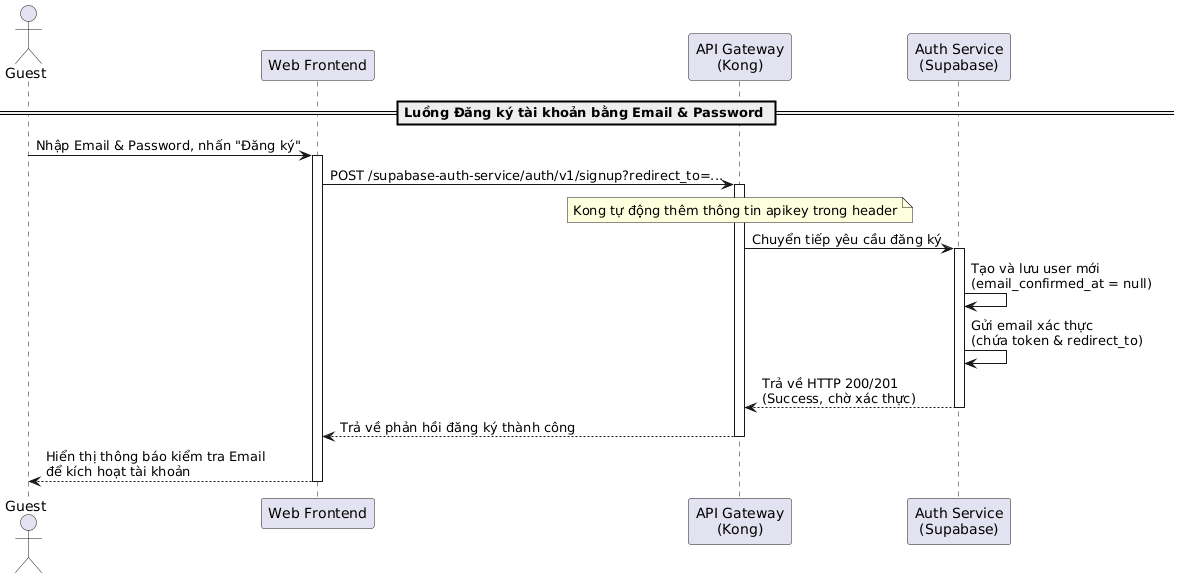
\includegraphics[scale = 0.35]{contents/Sequence/UML-Sequence-GuestEmailPasswordSignup.png}
\caption{Sơ đồ tuần tự luồng đăng ký tài khoản bằng email}
\end{figure}

\subparagraph{Các thành phần tham gia}

\begin{table}[H]
\centering
\renewcommand{\arraystretch}{1.3}

\begin{tabular}{|l|l|p{5cm}|}
\hline
\textbf{Thành phần} & \textbf{Phân loại} & \textbf{Vai trò trong hệ thống} \\ \hline
Guest & Actor & Khách vãng lai thực hiện đăng ký tài khoản mới. \\ \hline
Web Frontend & Component & Giao diện web Next.js. \\ \hline %%%% Component & Giao diện tiếp nhận thông tin đăng ký từ Guest. \\ \hline
API Gateway (Kong) & Component & Cổng API chuyển tiếp các yêu cầu API. \\ \hline %%%% Component & Cổng kết nối trung gian chuyển tiếp yêu cầu đăng ký đến Auth Service. \\ \hline
Auth Service (Supabase) & Microservice & Dịch vụ xác thực xử lý yêu cầu đăng ký, tạo tài khoản mới ở trạng thái chờ kích hoạt và gửi email xác thực. \\ \hline
\end{tabular}
\caption{Các thành phần tham gia luồng đăng ký tài khoản bằng email}
\end{table}

\subparagraph{Mô tả tổng quan}

\begin{itemize}
\item Guest nhập địa chỉ Email và mật khẩu, nhấn nút Đăng ký trên Web Frontend.
\item Web Frontend gửi yêu cầu đăng ký thông qua API Gateway. API Gateway định tuyến và chuyển tiếp yêu cầu đến Auth Service.
\item Auth Service tự động tạo và lưu thông tin người dùng mới với trạng thái chưa kích hoạt (\texttt{email\_confirmed\_at = null}).
\item Auth Service thực hiện gửi email xác thực chứa mã xác nhận (token) và liên kết chuyển hướng đến cho Guest.
\item Auth Service phản hồi kết quả đăng ký thành công (chờ xác thực) về Web Frontend thông qua API Gateway.
\item Web Frontend hiển thị thông báo yêu cầu Guest kiểm tra hòm thư điện tử để xác thực và kích hoạt tài khoản.
\end{itemize}
